\documentclass[11pt]{article}

\usepackage[margin=1in]{geometry}
\usepackage[T1]{fontenc}
\usepackage[utf8]{inputenc}
\usepackage{lmodern}
\usepackage{amsmath}
\usepackage{booktabs}
\usepackage{array}
\usepackage{longtable}
\usepackage{graphicx}
\usepackage{hyperref}
\usepackage{xcolor}
\usepackage{enumitem}

\hypersetup{
  colorlinks=true,
  linkcolor=blue,
  urlcolor=blue,
  citecolor=blue
}

\title{Building a Reproducible Numerai Quant-ML Research Pipeline}
\author{Nandhu Raj}
\date{June 2026}

\begin{document}
\maketitle

\begin{abstract}
This document summarizes the design and iteration history of a reproducible Numerai research pipeline for cross-sectional tabular prediction. The project began as a simple LightGBM baseline and evolved into a multi-model experiment system with era-aware walk-forward validation, feature exposure diagnostics, post-prediction neutralization, cached ensemble reblending, live prediction generation, and dry-run submission support. The goal was not to claim profitability, but to build a practical research workflow that reflects realistic quant-ML and ML engineering practice. The current best completed result is a medium-scale MLX-inclusive ensemble run with mean CORR 0.082707 and Sharpe-like score 1.262571. This writeup focuses on what was implemented, the failures encountered, the fixes applied, the alternative paths explored, and what the current results support.
\end{abstract}

\section{Project Goal}

The project objective was to build a Numerai pipeline that could support repeatable experimentation instead of one-off model runs. The intended workflow was:

\begin{enumerate}[leftmargin=1.5em]
  \item download Numerai tournament data without committing raw files;
  \item train baseline and alternative tabular models;
  \item validate them with era-aware walk-forward backtesting;
  \item generate live predictions in Numerai submission format;
  \item support dry-run-first submission through environment variables rather than hardcoded credentials;
  \item leave behind reproducible artifacts, plots, and reports after every run.
\end{enumerate}

The emphasis was therefore on making the research loop systematic, inspectable, and reusable rather than relying on a single model run.

\section{Problem Setting}

Numerai provides obfuscated market data with anonymous features, an \texttt{era} column, row identifiers, and a target. The practical modeling task is to predict the target cross-sectionally while respecting the time-like structure implied by eras. Since the features are anonymized, domain-specific feature engineering is limited. That naturally shifts the emphasis toward:

\begin{itemize}[leftmargin=1.5em]
  \item validation design,
  \item model comparison,
  \item ensemble construction,
  \item exposure control,
  \item and workflow discipline.
\end{itemize}

The project used the Numerai dataset version \texttt{v5.2} and local experiments were primarily run under Python 3.12 with \texttt{uv} for environment management.

\section{System Design}

\subsection{Repository Structure}

The repository was organized as a small Python package rather than a notebook-first project. Core logic lives under \texttt{src/numerai\_quant/}, command-line entry points live under \texttt{scripts/}, experiment settings live under \texttt{configs/}, and run outputs are written into ignored \texttt{artifacts/}, \texttt{models/}, and \texttt{data/} directories.

\subsection{Implemented Components}

The final system includes:

\begin{itemize}[leftmargin=1.5em]
  \item Numerai data download through \texttt{numerapi};
  \item automatic feature detection from columns prefixed with \texttt{feature\_};
  \item LightGBM, XGBoost, CatBoost, and MLX-based MLP model support;
  \item walk-forward fold generation using ordered eras, embargo periods, and configurable fold counts;
  \item validation metrics including era-wise Spearman correlation, mean correlation, standard deviation, Sharpe-like score, drawdown-style diagnostic, and feature exposure;
  \item post-prediction neutralization against highly exposed features;
  \item saved checkpoints and partial artifacts for interrupted runs;
  \item cached reblending from stored fold predictions without retraining base models;
  \item final ensemble bundle export for live inference;
  \item live prediction formatting and dry-run submission flow.
\end{itemize}

\section{Validation Protocol}

Validation was the central methodological choice in the project. Instead of using random train/validation splits, the pipeline treats \texttt{era} as a time-like grouping and evaluates models in a walk-forward fashion:

\begin{enumerate}[leftmargin=1.5em]
  \item train on earlier eras;
  \item skip an embargo gap to reduce leakage;
  \item validate on later eras;
  \item repeat across multiple folds.
\end{enumerate}

This does not eliminate all backtest risk, but it is far more defensible than independent and identically distributed splits for this setting.

For fast local iteration, many experiments used a medium validation budget with 3 folds and 4 validation eras per fold, yielding 12 validation eras in total. Later, stronger benchmark configurations were added with 15 folds and the same 4-era validation window, yielding 60 validation eras.

\section{Experiment Chronology}

\subsection{Stage 1: Baseline Trees}

The project started with LightGBM as the baseline system. This established the initial pipeline shape: loading parquet data, auto-detecting feature columns, training on the Numerai target, and producing rank-normalized predictions in the valid range.

Two LightGBM variants were retained in the model zoo:

\begin{itemize}[leftmargin=1.5em]
  \item \texttt{lgbm\_main}, which became the stable tree baseline;
  \item \texttt{lgbm\_alt}, which provided a weaker but still useful alternative signal for ensembles.
\end{itemize}

\subsection{Stage 2: XGBoost Branch}

The next experiment branch added XGBoost as a third model family. On the medium-scale validation setup, the XGBoost run produced:

\begin{center}
\begin{tabular}{lrr}
\toprule
Model & Mean CORR & Sharpe-like \\
\midrule
ensemble & 0.075227 & 1.084128 \\
xgb\_optional & 0.071617 & 1.185753 \\
lgbm\_main & 0.070495 & 1.045938 \\
lgbm\_alt & 0.052972 & 0.977822 \\
\bottomrule
\end{tabular}
\end{center}

This was a meaningful improvement over the original LightGBM-only setup and established that a model zoo plus ensembling was already better than a single-model baseline.

\subsection{Stage 3: CatBoost Branch}

CatBoost was then added as another alternative model family. Early CatBoost settings underperformed badly. A representative early medium run yielded:

\begin{center}
\begin{tabular}{lrr}
\toprule
Model & Mean CORR & Sharpe-like \\
\midrule
lgbm\_main & 0.070495 & 1.045938 \\
ensemble & 0.068955 & 1.044147 \\
ensemble\_neutralized & 0.067549 & 1.015856 \\
lgbm\_alt & 0.052972 & 0.977822 \\
catboost\_optional & 0.038138 & 1.067775 \\
\bottomrule
\end{tabular}
\end{center}

That poor first result was useful because it forced parameter iteration instead of letting the project tell an overly tidy story. After tuning, the CatBoost branch improved substantially:

\begin{center}
\begin{tabular}{lrr}
\toprule
Model & Mean CORR & Sharpe-like \\
\midrule
catboost\_optional & 0.079392 & 0.928660 \\
ensemble & 0.078841 & 1.015293 \\
ensemble\_neutralized & 0.077548 & 0.994846 \\
lgbm\_main & 0.070495 & 1.045938 \\
lgbm\_alt & 0.052972 & 0.977822 \\
\bottomrule
\end{tabular}
\end{center}

At this point CatBoost became the strongest standalone non-LightGBM model in the repository.

\subsection{Stage 4: Cached Reblending}

One of the strongest engineering improvements in the project was not a new model at all. It was cached reblending.

The walk-forward pipeline had already been modified to save fold-level prediction checkpoints. Building on that, a new workflow was added to recompute ensemble results from stored fold predictions without retraining any base models. This made it much cheaper to test new weights and blend strategies.

Optimizing the CatBoost-heavy blend on cached predictions produced:

\begin{center}
\begin{tabular}{lrr}
\toprule
Model & Mean CORR & Sharpe-like \\
\midrule
ensemble & 0.081843 & 0.972208 \\
ensemble\_neutralized & 0.080924 & 0.957781 \\
catboost\_optional & 0.079392 & 0.928660 \\
lgbm\_main & 0.070495 & 1.045938 \\
lgbm\_alt & 0.052972 & 0.977822 \\
\bottomrule
\end{tabular}
\end{center}

The best optimized CatBoost reblend chose weights:
\[
\texttt{lgbm\_main} = 0.30, \quad
\texttt{lgbm\_alt} = 0.00, \quad
\texttt{catboost\_optional} = 0.70
\]

This was an important moment in the project because it showed that workflow improvements could create measurable modeling gains.

\subsection{Stage 5: Feature Filtering Experiments}

The project also explored simple feature-selection and redundancy-control paths, including:

\begin{itemize}[leftmargin=1.5em]
  \item correlation pruning;
  \item importance-based top-\(N\) filtering.
\end{itemize}

These were implemented cleanly and evaluated, but in practice they hurt performance on the medium validation setup. That result is worth documenting because it prevented unnecessary complexity from becoming permanent just because it sounded sophisticated.

\subsection{Stage 6: MLX Neural Branch}

Because the hardware environment included Apple Silicon, the project added an MLX-based MLP path as a neural tabular experiment lane.

The first MLX attempt was weak. Later versions improved sharply, especially after the training loop was aligned more closely with Numerai validation:

\begin{itemize}[leftmargin=1.5em]
  \item early stopping on the actual fold validation set instead of only a random internal split;
  \item support for validation based on era-wise correlation rather than only MSE;
  \item input noise and larger hidden layers in later configurations.
\end{itemize}

An improved MLX-inclusive run produced:

\begin{center}
\begin{tabular}{lrr}
\toprule
Model & Mean CORR & Sharpe-like \\
\midrule
ensemble & 0.082707 & 1.262571 \\
ensemble\_neutralized & 0.082453 & 1.234679 \\
lgbm\_main & 0.070495 & 1.045938 \\
mlx\_mlp\_optional & 0.058747 & 3.461954 \\
lgbm\_alt & 0.052972 & 0.977822 \\
\bottomrule
\end{tabular}
\end{center}

This was the best completed ensemble score observed in the project. However, the MLX model itself was not the strongest standalone learner. Its value appeared to come from diversification rather than raw standalone accuracy.

When the same MLX branch was optimized with cached reblending, the result fell to:

\begin{center}
\begin{tabular}{lrr}
\toprule
Model & Mean CORR & Sharpe-like \\
\midrule
ensemble & 0.080167 & 1.170258 \\
ensemble\_neutralized & 0.079942 & 1.143904 \\
lgbm\_main & 0.070495 & 1.045938 \\
mlx\_mlp\_optional & 0.058747 & 3.461954 \\
lgbm\_alt & 0.052972 & 0.977822 \\
\bottomrule
\end{tabular}
\end{center}

The optimized weights for that branch were:
\[
\texttt{lgbm\_main} = 0.55, \quad
\texttt{lgbm\_alt} = 0.05, \quad
\texttt{mlx\_mlp\_optional} = 0.40
\]

This made the MLX branch more interesting, not less. It suggested that the neural model may be adding useful but less stable diversity, rather than providing a robust replacement for the tree-based baseline.

\section{Engineering Issues Encountered and Fixes Applied}

The repository improved substantially through debugging and workflow repair, not only through model tuning.

\subsection{Data Download Friction}

Initially, the downloader pulled train, validation, and live files sequentially every time. That created unnecessary waiting and made failures harder to reason about. The data workflow was revised to:

\begin{itemize}[leftmargin=1.5em]
  \item support selective flags such as \texttt{--train-only}, \texttt{--validation-only}, and \texttt{--live-only};
  \item separate dependency-aware steps so backtests can start as soon as training data is ready;
  \item log clear start and finish messages around each file;
  \item reuse a single NumerAPI client.
\end{itemize}

\subsection{Interrupted Runs and Partial Progress}

Long runs on a laptop and in Colab were vulnerable to crashes, disconnects, and sleep-related interruptions. To reduce wasted time, the pipeline was extended to write:

\begin{itemize}[leftmargin=1.5em]
  \item partial fold metrics;
  \item partial OOF predictions;
  \item fold checkpoints;
  \item run status metadata.
\end{itemize}

This made it much easier to inspect what had completed and enabled the later reblend workflow.

\subsection{Identifier and Index Handling}

At one point the backtest failed with a missing \texttt{id} column error. The root cause was that some frames treated the identifier as an index rather than a normal column. The fix was to centralize identifier handling in a helper that promotes the index to a named identifier column when needed.

\subsection{Backend and Compatibility Issues}

The project also hit a plotting backend failure in Colab because \texttt{matplotlib\_inline} was being inherited as a backend value unsupported by the package configuration in that environment. The initialization path was updated to behave more safely in notebook and Colab-style contexts.

Another small but disruptive issue came from using a \texttt{reset\_index(names=...)} pattern that was not supported in the runtime mix actually used during execution. That was simplified to a more compatible approach.

\subsection{MLX Validation Mismatch}

The early MLX implementation used a random internal validation split with MSE-based early stopping. That was a poor match for the actual evaluation target. The fix was to let the MLX trainer use the fold validation slice directly and to support era-wise correlation as the validation signal.

\section{What the Results Support Right Now}

The current repository supports several honest claims:

\begin{enumerate}[leftmargin=1.5em]
  \item The project is no longer a toy notebook. It is a reproducible, config-driven ML research pipeline.
  \item Era-aware backtesting was implemented correctly enough to make model comparisons more credible than random-split baselines.
  \item Ensembling across model families was useful, and cached reblending improved iteration speed substantially.
  \item CatBoost became the strongest stable tree-based alternative beyond LightGBM.
  \item MLX-based neural models became competitive enough to improve the best completed ensemble result, even if they are not yet the most stable branch.
\end{enumerate}

At the same time, the repository does \emph{not} support stronger claims such as:

\begin{itemize}[leftmargin=1.5em]
  \item proven profitability;
  \item live robustness;
  \item production-grade monitoring;
  \item or a definitive statement that the neural branch is superior to the tree branch.
\end{itemize}

The best completed run still uses 12 validation eras, which is useful for iteration and model comparison but narrower than the stronger benchmark configurations that have also been prepared.

\section{Alternative Paths Explored}

Several alternative directions were evaluated during the project:

\begin{itemize}[leftmargin=1.5em]
  \item \textbf{XGBoost branch:} useful and competitive, but ultimately overtaken by the best CatBoost configuration.
  \item \textbf{CatBoost branch:} initially weak, then improved enough to become the strongest stable branch.
  \item \textbf{Feature filtering:} implemented cleanly but not retained as a winning direction because it hurt scores.
  \item \textbf{Neural MLX branch:} more volatile than the tree-based alternatives, but valuable because it introduced a genuinely different signal family.
  \item \textbf{Manual vs. optimized blending:} both were informative. In the CatBoost branch, optimized reblending improved the score. In the MLX branch, the manual blend outperformed the optimizer, indicating lower stability.
\end{itemize}

\section{Operational Constraints}

The experiments were shaped by very real hardware and workflow constraints:

\begin{itemize}[leftmargin=1.5em]
  \item large parquet downloads are slow and storage-heavy;
  \item a MacBook Pro can run these experiments, but long multi-fold training creates thermal and unified-memory pressure;
  \item Colab can help, but session disconnects and ephemeral files make artifact persistence fragile unless runs are structured carefully.
\end{itemize}

Those constraints pushed the project toward a more disciplined approach to checkpointing, selective downloads, thread capping, and cached re-use of fold predictions.

\section{Current Best View of the System}

At the time of writing, the project has two strong research branches:

\begin{itemize}[leftmargin=1.5em]
  \item a \textbf{CatBoost-heavy branch}, which is the strongest stable benchmark path;
  \item an \textbf{MLX-inclusive branch}, which produced the best completed ensemble score but has not yet shown the same robustness under blend optimization.
\end{itemize}

The practical interpretation is:

\begin{itemize}[leftmargin=1.5em]
  \item CatBoost is the safer branch for a stronger benchmark run;
  \item MLX is the more experimental branch, worth keeping because it can add useful diversity.
\end{itemize}

\section{Next Steps}

The next steps are straightforward:

\begin{enumerate}[leftmargin=1.5em]
  \item run the 60-validation-era benchmark configurations and compare them against the current best completed medium-scale run;
  \item re-optimize blends on those stronger runs;
  \item decide whether the public benchmark should remain CatBoost-heavy or whether the MLX branch survives at larger scale;
  \item eventually track live submission behavior rather than only backtest outputs.
\end{enumerate}

\section{Conclusion}

This project started as a baseline Numerai modeling pipeline and improved through repeated iteration on both modeling and engineering. The most useful lesson was that experimentation infrastructure mattered as much as model choice. Better downloads, better checkpoints, better validation alignment, and cached reblending changed the pace and quality of iteration. The resulting system is not proof of alpha, but it is a credible applied research workflow for quant-ML and ML engineering practice.

\begin{figure}[t]
  \centering
  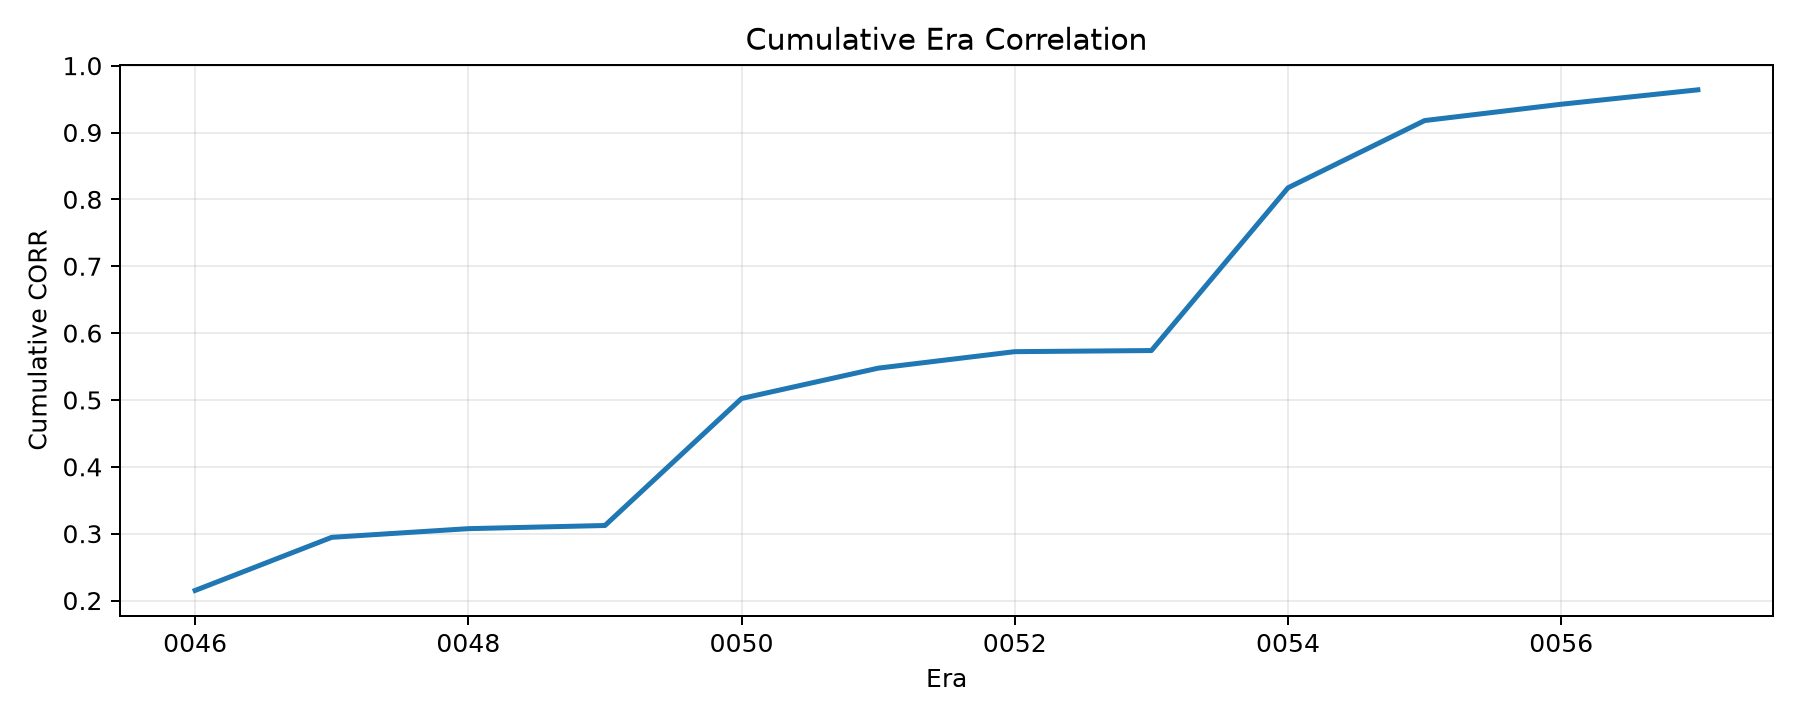
\includegraphics[width=0.9\textwidth]{sample_artifacts/best_medium_reblend/cumulative_corr.png}
  \caption{Cumulative era correlation from the curated medium-scale sample run.}
\end{figure}

\end{document}
